\documentclass[11pt,a4paper,oneside]{report}
\usepackage[utf8]{inputenc}
\usepackage[english]{babel}
\usepackage{amsmath}
\usepackage{amsfonts}
\usepackage{amssymb}
\usepackage{graphicx}
\usepackage[left=2cm,right=2cm,top=2cm,bottom=2cm]{geometry}
\author{Daniel Aguiar da Silva Carvalho}
\begin{document}
\sffamily
\begin{center}
\textbf{\large{Thesis Advancement Report 2014-2015 (First Year)}}
\end{center}

\begin{flushleft}
\textbf{Thesis title:} Trusted-SLA Guided Data Integration on Multi-cloud Environments \\
\textbf{PhD. student:} Daniel Aguiar da Silva Carvalho \\
\textbf{Supervisor:} Chirine Ghedira-Guegan \textbf{Co-supervisors:} Nadia Bennani and Genoveva Vargas-Solar 
\end{flushleft}

\begin{flushleft}
\textbf{1 Context}\footnote{You can find the references at https://www.dropbox.com/s/dyg08a622ucv6xl/references.pdf?dl=0} \\
\end{flushleft} 
The data integration is a well-known and widely studied problem in the database domain. 
It consists in merging data from different data sources and granting a unified view~\cite{Lenzerini:2002}. 
%
The main contributions of the area are: (i) providing a global  representation of heterogeneous data  by defining a schema (e.g., global and local as view approaches); (ii) tagging data with meta-data or by associating them to knowledge (e.g. semantic Web approaches); and (iii)   architectures used for integrating data (i.e. distributed databases, multi-databases,  federated databases, etc).
%
The emergence of cloud computing and service oriented computing opens new challenges to data integration. 
The possibility of an unlimited access to resources  changes the problems associated to data processing. Cloud-based data management using data sharing  enables the collaboration of different entities to perform design tasks \cite{Gonzalez:2010,Gonzalez:2010b}. Data processing and analytics are costly tasks that can benefit from the cloud elastic resources provision, coupled with  programming paradigms like Map-Reduce. \cite{078} proposes SODIM that works on a pool of collaborative services and can process a large number of databases represented as web services. 


In the cloud scenario resources are not necessarily located in the same cloud. One cloud cannot be expected to provide the necessary resources to fulfill application requirements. 
With growing needs and requirements, applications use different cloud providers for externalizing different data processing and management resources
adding more challenges to data integration, considering the large amount and diversity of data, user quality and security requirements of the integration, and cloud heterogeneity in expressing and enforcing the corresponding clauses~\cite{Dustdar:2012}.

In cloud computing, a common way of defining requirements and obligations between the \textit{provider} and \textit{customer} is through service level agreement (SLA). 
SLAs have been  adopted in the cloud, focussing (i) on the lifecycle of a security SLA on hybrid clouds~\cite{011}; (ii) on SLA models for addressing  management capabilities  as a service, Pcloud services, performed through agreed and negotiated in contracts (elasticity, high availability, scalability and on demand provisioning)~\cite{009}; and (iii) on functional and non-functional requirements of the different cloud delivery models~\cite{005}.
Summarizing, SLA contributions focus on: (i)   the SLA negotiation phase; and (ii)  resources monitoring and allocation  to detect and avoid SLA violations. We identified one single approach regarding data integration in a grid environment guided by SLA~\cite{Nie07}.

\begin{flushleft}
\textbf{2 Problem Statement}\\
\end{flushleft}
The problem addressed in our work is how can a user \textbf{efficiently} obtain results for her queries, \textbf{meeting her QoS requirements}, respecting all her subscribed contracts with the involved cloud provider(s), and without neglecting services contracts? 
Particularly, for queries that call several services deployed on different clouds.

\noindent
{\em Hypothesis:}  We assume that data are provided as services that export APIs with methods to retrieve  and process data. Data integration is done (i) on a (multi)-cloud service oriented environment;  (ii) under new conditions with respect to the type of data sources, the environment where it is performed and the preferences  of data consumers and the SLA. We assume also that (iii) SLA measures can be monitored and negotiated in all cloud providers; and that (iv) cloud services and data services are listed in a registry.

We believe that data integration on multi-cloud environments can take advantage by integrating SLA on its solutions. To the best of our knowledge, we have not identified any other proposal adopting the use of SLAs combined with a data integration approach on a (multi)-cloud context.

\begin{flushleft}
\textbf{3 Objectives}\\
\end{flushleft}
The  objective is to propose a data integration solution in a multi-cloud environment guided by user preferences and SLA exported by different clouds. This new approach brings different challenges and open issues: (1)  Identify and classify quality measures linked to data quality, data security and to cloud resources; (2) Propose an unified formalism to represent them; (3) Propose and implement a mechanism that ensures SLA within the data integration process  performed on a multi-cloud and cope this with application requirements; and (4) Design a new matching-retrieving algorithm to perform the integration process, selecting the best service composition according to the user requirements and the SLAs.
 
\begin{flushleft}
\textbf{4 Synthesis and Perspectives of the Research Activities}\\
\end{flushleft}
During the fist year we have organized our research activities in three groups (see below). These activities were organized and discussed in meetings with advisors and with individual work.

\noindent
\textbf{Problem statement and state of the art.} The objective has been to acquire background knowledge on data integration, cloud and SLA building a corpus with publications  and reading selected papers. Therefore, we applied the systematic mapping methodology consisting in retrieving papers from scientific databases,   filtering them according to inclusion and exclusion criteria and research interests expressed in research questions. A classification schema was  proposed, consisting in   facets and dimensions. The abstracts of the final papers collection were read  to classify each paper within the scheme.  We identified the trends and open issues in our research topic and proposed the general lines of  an original data integration solution according to current trends in the area.

\noindent
{\em Results:} We built a collection of 114 papers and analytics results. We proposed a data integration classification scheme that serves as initial entry for building a state of the art. 

\noindent
\textbf{Experimentation.} We are currently configuring an experimentation platform on the cloud using Open Stack to implement and evaluate our match-retrieving algorithm~\footnote{You can check the detailed list of activities in https://www.dropbox.com/s/2cf6gncumzrjacd/sla-matching-experiment.docx?dl=0}.

\noindent
\textbf{Publications and thematic schools.}

\noindent
D. A. S. Carvalho, P. A. Souza Neto, G. Vargas-Solar, N. Bennani, C. Ghedira, Can Data Integration Quality be Enhanced on Multi-cloud using SLA?, Short paper, {\em In Proceedings of the 26th International Conference on Database and Expert Systems Applications}, LNCS, Valencia, Spain, 2015 (to appear)

\noindent
Additionally, in April, I attended to the \emph{1st French Brazilian School on Smart cities and Big Data} at the University of Grenoble Alpes (http://fr-br-school.imag.fr).

\noindent
The figure below presents the perspectives described as activities in the following calendar. 

\begin{figure}[!b]
\center
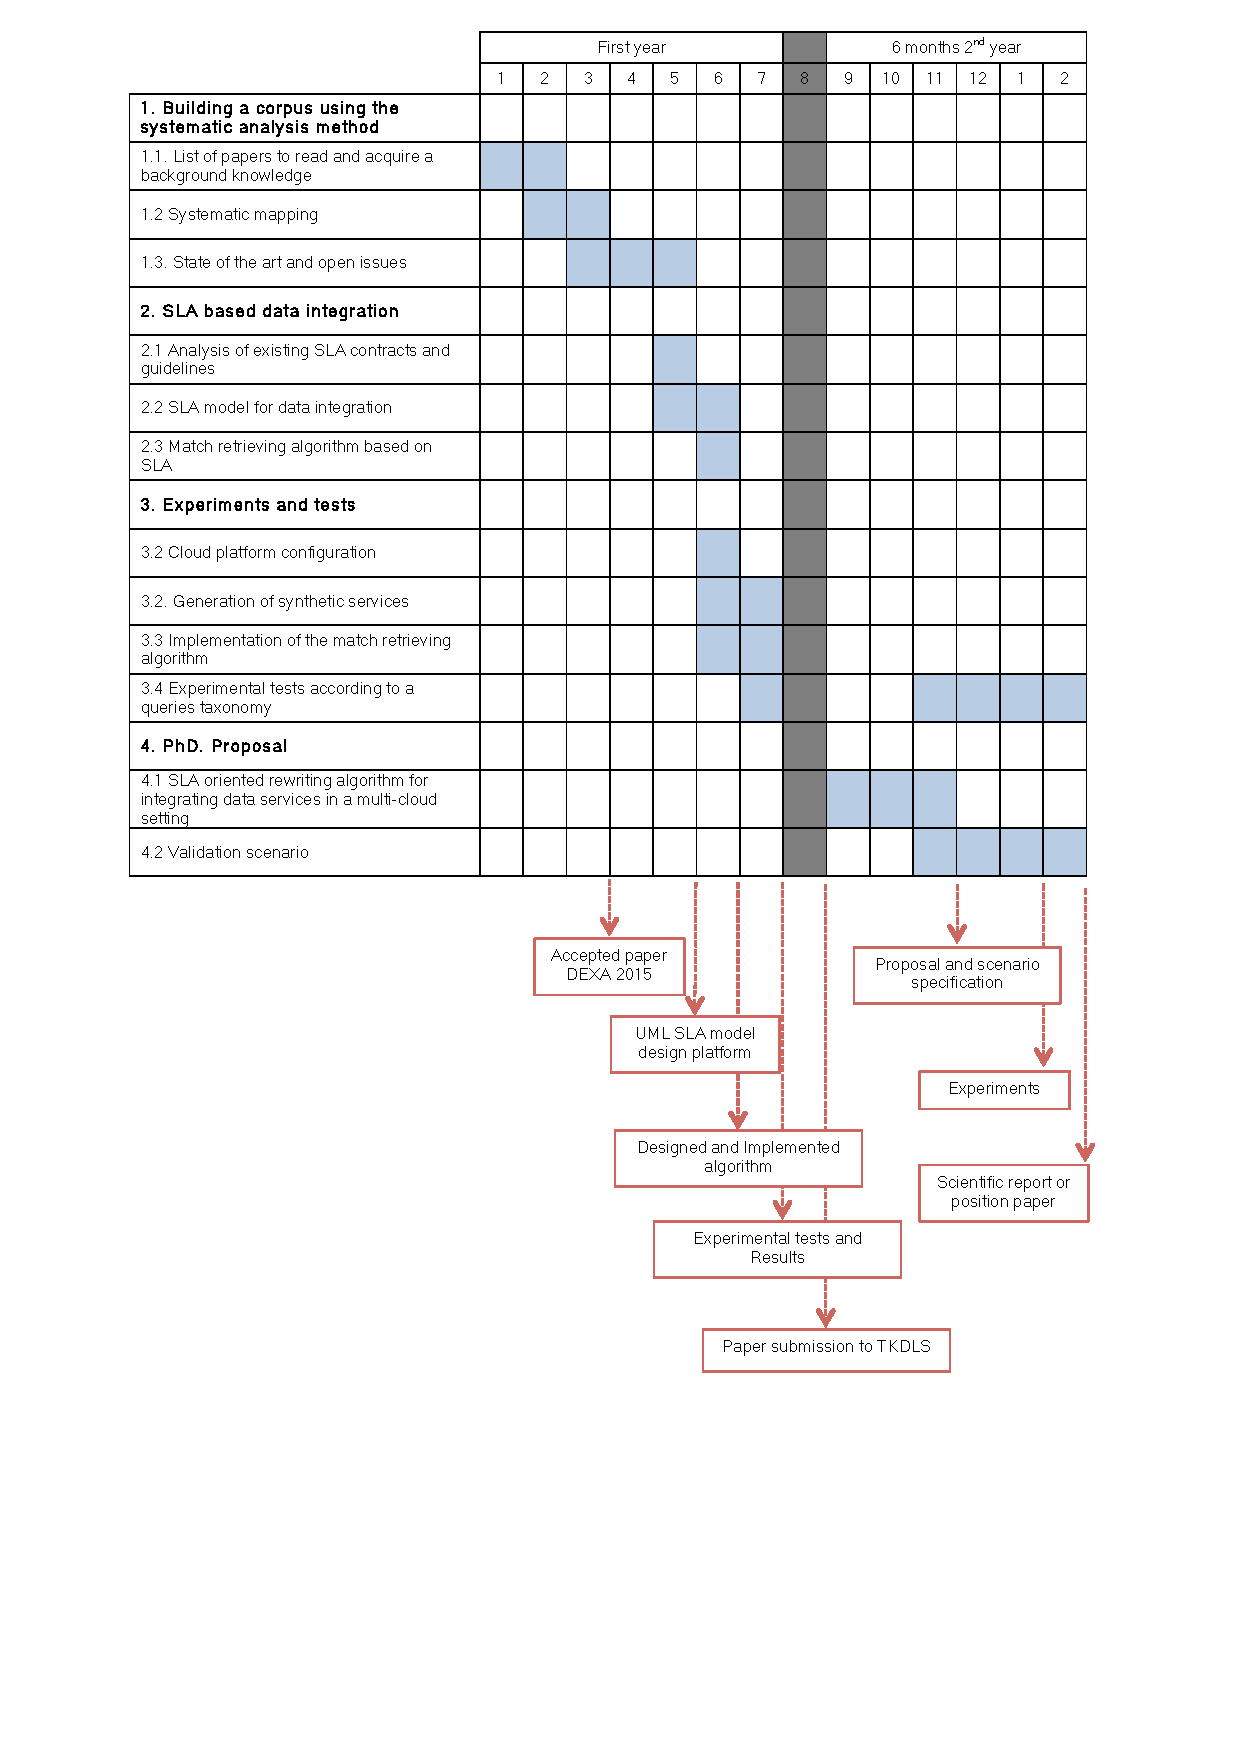
\includegraphics[scale=0.37]{calendario.png}
\end{figure}

\bibliographystyle{plain}
\bibliography{bibliography}


\end{document}